\documentclass{article}
\usepackage{amsmath}
\usepackage{pgfplots}

\setlength\parindent{0pt}

\pgfkeys{/pgfplots/MyAxisStyle/.style={xmin=-10,xmax=10, ymin=-10,ymax=10,height=6cm,width=6cm}}

\begin{document}

\section*{Previously}

We covered the idea that the closed line integral is zero always, however, there are different situations where this is not true.

\[
\int_c \vec{F}\cdot d\vec{s} = 0
\]

where $c$ is a closed curve.

\hrulefill

\section*{\# 27}

We want to calculate the integral

\[
\int_c \vec{F}\cdot d\vec{s}
\]

Where $c$ is a simple circle of radius $r$ centered at the origin.

\[
\vec{F} = \left<-\dfrac{y}{x^2+y^2}, \dfrac{x}{x^2+y^2}\right>
\]

It's easy to show that

\[
\dfrac{\partial F_1}{\partial y} = \dfrac{\partial F_2}{\partial x}
\]

Which would seem to tell us that the integral should be zero, by the fundamental thereom.

However, the curve $c$ can also be given by

\[
c: \begin{cases}
  x = r \cos{\theta} \\
  y = r \sin{\theta} \\
  0 \le \theta \le 2\pi
\end{cases}
\]

Plugging into the formula we get

\[
\int_c -\dfrac{y}{x^2+y^2} dx + \dfrac{x}{x^2+y^2} dy
\]

\[
= \int_0^{2\pi} \left[-\dfrac{r \sin{\theta}}{r^2} \left(-r \sin{\theta}\right) + \dfrac{r \cos{\theta}}{r^2} \left(r \cos{\theta}\right)\right] d\theta
\]

\[
= \int_0^{2\pi} 1 d\theta = 2\pi
\]

How do we make sense of this? The fundamental theorem gives one solution, and this other method gives a difference solution?

The original function includes a discontinuous point at $(x,y)=(0,0)$, but we can remove that by the following:

We can take our original circle $c$ and modify the shape so that it does not contain the discontinuous point, which would give the expected value of zero.

%\draw(0,0) circle(1)
%\draw(0,0) circle(0.5)
%\line between circles at y=-0.2
%\line between circles at y=0.2

\hrulefill

\section*{17.1}
\subsection*{Green's Theorem}

We'll be focusing on type 2 line integrals (vector integrals) around a closed curve.

\[
\oint_c \vec{F}\cdot d\vec{s}
\]

We need to define the direction of this closed curve as taking positive to mean counter-clockwise.

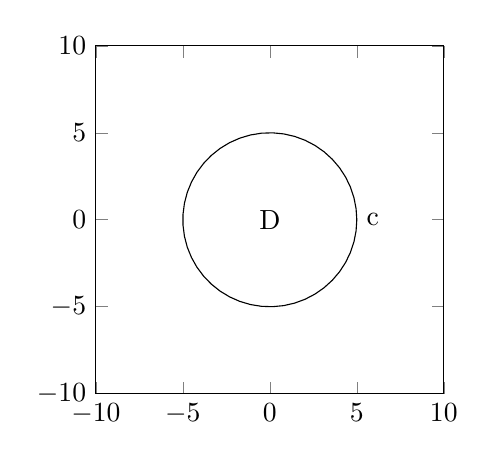
\begin{tikzpicture}
  \begin{axis}[MyAxisStyle]
    \addplot [domain=0:2*pi,samples=50] ({5*cos(deg(x))},
                                         {5*sin(deg(x))});
    \draw (axis cs:0,0) node{D};
    \draw (axis cs:5,0) node[right]{c};
  \end{axis}
\end{tikzpicture}

\subsection*{Thereom: Green's Theorem}

\[
\oint_c \vec{F}\cdot d\vec{s} = \int \int_D \dfrac{\partial F_2}{\partial x} - \dfrac{\partial F_1}{\partial y} dA
\]

\subsection*{Remark}

Notice that, in the case of conservativity, the left side is supposed to be zero, by the fundamental thereom. In that case, the difference

\[
\dfrac{\partial F_2}{\partial x} = \dfrac{\partial F_1}{\partial y}
\]

Causing

\[
\oint_c \vec{F}\cdot d\vec{s} = 0
\]

\section*{Example}

Suppose that

\[
\vec{F} = \left<\sin{x}, x^2 y^3\right>
\]

and $c$ can be given by

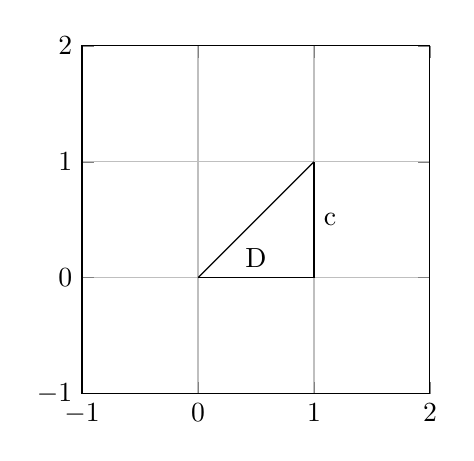
\begin{tikzpicture}
  \begin{axis}[MyAxisStyle,xmin=-1,xmax=2,ymin=-1,ymax=2,grid=major]
    \draw (axis cs:0,0) -- (axis cs:1,0);
    \draw (axis cs:1,0) -- (axis cs:1,1);
    \draw (axis cs:1,1) -- (axis cs:0,0);
    \draw (axis cs:0.5,0) node[above]{D};
    \draw (axis cs:1,0.5) node[right]{c};
  \end{axis}
\end{tikzpicture}

We want to calculate

\[
\oint_c \vec{F}\cdot d\vec{s}
\]

Normally, we'd have three line integrals, but with Green's Thereom, we only have to do one double integral.

\[
=\int \int_D 2 x y^3 - 0 dA
\]

\[
=\int_0^1 \int_0^x 2 x y^3 dy dx
\]

\[
=\int_0^1 2 x \left[\frac{1}{4} y^4 \right]_{y=0}^{y=x} dx
\]

\[
=\frac{1}{12}
\]

\hrulefill

\section*{Example}

\[
\oint_c \underset{F_1}{\left[y+\sqrt{1+x^4}\right]} dx + \underset{F_2}{\left[2x+e^{\sin y}\right]} dy
\]

Normally, this would be very difficult to calculate the antiderivative of these functions, but we can use Green's Theorem to more easily calculate the integral.

\[
=\int \int_D \left[2 - 1\right] dA
\]

\[
=\pi
\]

\hrulefill

\section*{Example: \#26}

\[
\oint_c \dfrac{-y}{x^2+y^2} dx + \dfrac{x}{x^2+y^2} dy
\]

This looks like it would be nice, but the function is discontinuous at $(x,y)=(0,0)$. We let $c$ be a curve which does not enclose the origin.

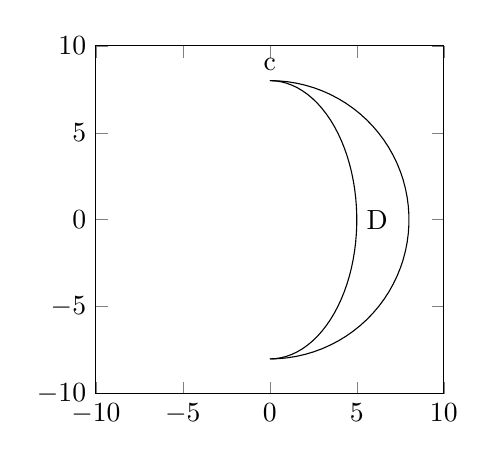
\begin{tikzpicture}
  \begin{axis}[MyAxisStyle]
    \addplot [domain=-pi/2:pi/2,samples=50] ({8*cos(deg(x))},
                                             {8*sin(deg(x))});
    \addplot [domain=-pi/2:pi/2,samples=50] ({5*cos(deg(x))},
                                             {8*sin(deg(x))});
    \draw (axis cs:0,8) node[above]{c};
    \draw (axis cs:5,0) node[right]{D};
  \end{axis}
\end{tikzpicture}

\[
=\int \int_D \left[ Something - Something \right] dA
\]

\[
=0
\]

\hrulefill

\section*{When would we use Green's Thereom?}

We would use it when we have a nice domain under the closed curve. Additionally, any time we are given a weird integrand, then Green's Thereom might simplify the integrand.

We can also go backwards, and compute a double integral with a line integral.

\section*{Applications of Green's Theorem: Area}

Where $c$ is a closed surface with $D$ enclosed.

\[
\dfrac{1}{2} \oint \underset{F_1}{-y} dx + \underset{F_2}{x} dy
\]

\[
=\dfrac{1}{2} \int \int \left[1 - \left(-1\right)\right] dA
\]

\[
=\text{Area of $D$}
\]

\[
\text{Area of $D$} = \dfrac{1}{2} \oint_c -y dx + x dy
\]

\section*{Example}

Given an ellipse with major axis radius of $a$ and minor axis radius of $b$, such that it can be described by

\[
\dfrac{x^2}{a^2}+\dfrac{y^2}{b^2}=1
\]

\[
\begin{cases}
  x = a \cos{\theta} \\
  y = b \sin{\theta} \\
  0 \le \theta \le 2 \pi
\end{cases}
\]

\[
\text{Area of $D$} = \dfrac{1}{2} \int_0^{2\pi} \left(-b \sin{\theta}\right) \left(-a \sin{\theta}\right) + \left(a \cos{\theta} b \cos{\theta}\right) d\theta
\]

\[
= \dfrac{1}{2} \left[a b \right]_0^{2\pi} = \pi a b
\]

\section*{Homework}

16.3 and 17.1

\end{document}
